\section{Variational Autoencoders}

Learning useful representations without labels requires us to tell the model what ``useful'' means. Variational autoencoders (VAEs) formalize this request by combining the information-theoretic appeal of autoencoders with explicit probabilistic modeling. This chapter develops VAEs from the bottom up: we motivate the desiderata for unsupervised representations, examine why maximizing mutual information alone fails, cast autoencoders in a Bayesian light, derive the evidence lower bound (ELBO), and describe how to optimize it in practice.

\subsection{Representation learning without supervision}
Deep networks can be viewed as compositions of an \emph{encoder} that maps the input $x \in \mathcal X$ into a latent representation $z$ and a \emph{decoder} (or predictor) that turns $z$ into a task output. When no labels are available, the only supervision we can provide is the input itself. Good representations should therefore satisfy three properties:
\begin{description}
    \item[Informative.] The original input should be recoverable from $z$, so no essential information is discarded.
    \item[Disentangled.] Individual coordinates of $z$ should align with distinct generative factors (pose vs.\ lighting, stroke width vs.\ digit identity, \emph{etc.}), enabling controlled manipulation.
    \item[Robust.] Small perturbations in the input should not cause drastic changes in $z$, and conversely modifying $z$ slightly should not flip the reconstruction arbitrarily.
\end{description}
Autoencoders optimize informativeness by minimizing reconstruction error, but disentanglement and robustness typically require further regularization.

\subsection{The infomax principle and its limitations}
Let $\text{enc}_\theta \in \mathcal H$ be a (possibly stochastic) encoder. The infomax principle (Linsker, 1988) advocates selecting the parameters $\theta$ that maximize the mutual information $I(X; Z)$ between inputs $X$ and their representations $Z=\text{enc}_\theta(X)$:
\[
I(X; Z) = \int p(x, z) \log \frac{p(x, z)}{p(x)\, p(z)}\, dx\, dz 
\]
With only data $x_1, \ldots, x_n$, the expectation can be approximated via Monte Carlo:
\[
I(X; Z) \approx \sum_{i \leq n} \mathbb{E}_{Z \mid x_i}\left[\log p\left(x_i \mid Z\right)\right]
\]
which resembles the reconstruction score of an autoencoder. Unfortunately, maximizing $I(X; Z)$ alone can be trivial whenever $\mathcal X$ and $\mathcal Z$ are rich enough: the encoder can simply implement a bijection (or memorize the dataset) so that $Z$ is a lossless copy of $X$. Such degenerate solutions are perfectly informative but neither disentangled nor robust, underscoring the need for additional inductive biases.

\subsection{Latent-variable generative modeling}
To go beyond empty informativeness, we posit a generative story for the data. A latent variable $Z$ is sampled from a prior $p(z)$, and the observation $X$ is drawn from a conditional decoder $p_\theta(x \mid z)$. This \emph{decoder} can be a deep neural network that outputs the parameters of a likelihood distribution (Gaussian for continuous data, Bernoulli/Categorical for binary or discrete data). High-quality representations now correspond to posterior inferences: given $x$, infer the distribution $p_\theta(z \mid x)$ of latent causes. Integrating the latent variable out gives the marginal likelihood $p_\theta(x) = \int p_\theta(x \mid z) p(z)\, dz$, which quantifies how well the generative model explains the observation.

Two conceptual benefits arise:
\begin{itemize}
    \item Sampling new $x$ is straightforward: draw $z \sim p(z)$ and decode it. VAEs thus act as generative models capable of ``hallucinating'' plausible data such as handwritten digits or faces.
    \item Regularization becomes Bayesian: the prior $p(z)$ codifies which representations are plausible (e.g., standard normal means centered, isotropic latent factors), discouraging memorization.
\end{itemize}
The main obstacle is posterior inference. Computing $p_\theta(z \mid x)$ exactly is typically intractable because it requires normalizing the product $p_\theta(x \mid z)p(z)$ over all $z$. Variational inference circumvents this by introducing an auxiliary encoder $q_\phi(z \mid x)$, parameterized by $\phi$, that approximates the true posterior.

\subsection{A manifold perspective}
High-dimensional data often concentrate near a \emph{manifold}---a smooth, low-dimensional surface embedded in the ambient space. Pictures of faces, for instance, span thousands of pixels yet vary along a handful of semantic axes such as pose, lighting, and expression. VAEs can be interpreted as tools for learning coordinates on this manifold. The decoder $p_\theta(x \mid z)$ acts like a chart that maps latent coordinates $z$ into points on (or near) the data manifold, while the encoder $q_\phi(z \mid x)$ performs the inverse mapping from observations back to manifold coordinates. The prior $p(z)$ then regularizes the geometry of this manifold by favoring latents near the origin, which in turn encourages smooth, disentangled directions. Thinking in manifold terms clarifies why VAEs produce interpolations that remain realistic: straight lines in latent space correspond to geodesic-like curves on the learned manifold, yielding gradual transitions in pixel space.

\begin{figure}[ht]
    \centering
    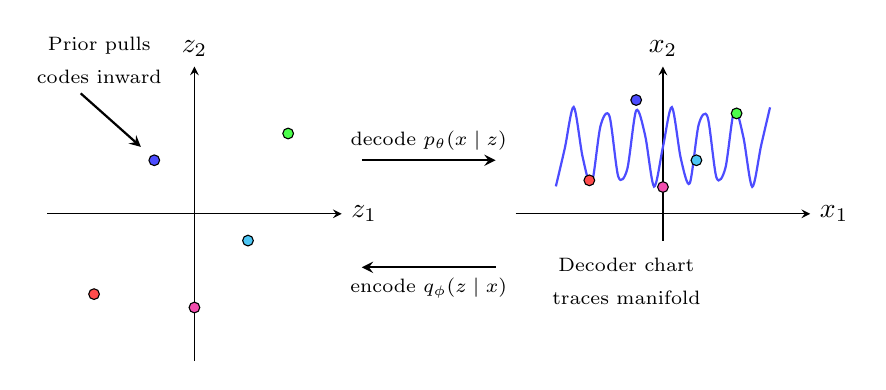
\begin{tikzpicture}[scale=0.85, >=stealth]
        % Latent space axes
        \begin{scope}
            \draw[->] (-2.2,0) -- (2.2,0) node[right] {$z_1$};
            \draw[->] (0,-2.2) -- (0,2.2) node[above] {$z_2$};
            % \node at (0,2.5) {\small Latent space $z$};
            \foreach \x/\y/\c in { -1.5/-1.2/red, -0.6/0.8/blue, 0.8/-0.4/cyan, 1.4/1.2/green, 0.0/-1.4/magenta} {
                \filldraw[fill=\c!70, draw=black] (\x,\y) circle (0.08);
            }
            \draw[->, thick] (-1.7,1.8) -- (-0.8,1.0);
            \node[align=center, anchor=south west] at (-2.5,1.8) {\scriptsize Prior pulls\\\scriptsize codes inward};
        \end{scope}
        % Decoder arrow
        \draw[->, thick] (2.5,0.8) -- (4.5,0.8) node[midway, above] {\scriptsize decode $p_\theta(x\mid z)$};
        % Data manifold axes
        \begin{scope}[xshift=7cm]
            \draw[->] (-2.2,0) -- (2.2,0) node[right] {$x_1$};
            \draw[->] (0,-0.4) -- (0,2.2) node[above] {$x_2$};
            % \node at (0,2.5) {\small Data manifold in $x$};
            % Manifold curve
            \draw[thick, blue!70] plot [smooth, domain=-1.6:1.6] (\x,{1 + 0.6*sin(\x r * 60)});
            % Points mapped
            \foreach \x/\y/\c in { -1.1/0.5/red, -0.4/1.7/blue, 0.5/0.8/cyan, 1.1/1.5/green, 0.0/0.4/magenta} {
                \filldraw[fill=\c!70, draw=black] (\x,\y) circle (0.08);
            }
            \node[align=center, anchor=south west] at (-1.8,-1.5) {\scriptsize Decoder chart\\\scriptsize traces manifold};
        \end{scope}
        % Encoder arrow
        \draw[<-, thick] (2.5,-0.8) -- (4.5,-0.8) node[midway, below] {\scriptsize encode $q_\phi(z\mid x)$};
    \end{tikzpicture}
    \caption{The encoder learns manifold coordinates while the decoder maps latent points back onto the curved data manifold, keeping interpolations smooth.}
    \label{fig:vae_manifold}
\end{figure}

\subsection{A Bayesian detour}
Bayesian estimation provides intuition for why priors help disentangle noise from signal. Suppose we wish to estimate the mean shoe size $\mu$ in a small town. A Gaussian prior $\mu \sim \mathcal N(\alpha, \beta)$ captures our belief before collecting data. Observing measurements $x_1, \ldots, x_n$ with $x_i \sim \mathcal N(\mu, 1)$ yields a Gaussian posterior $\mathcal N(\mu \mid m, s^2)$ that balances the prior and the evidence. When few samples are available, the posterior stays near $\alpha$ (robustness to noise); as $n$ grows, the data dominate (informativeness). VAEs apply the same logic in every latent dimension: the prior $p(z)$ nudges encodings toward structured, disentangled regions while still allowing the decoder to reconstruct the input accurately.
